\chapter{Experiment and Result}
brief of experiment and result.
\section{Experiment}
Please tell how the experiment conducted from method.

\section{Result}
Please provide the result of experiment

\section{Lusia Violita Aprilian/1164080}

\subsection{Teori}
\begin{enumerate}
\item Klasifikasi teks
	\par Klasifikasi Dokumen / Teks adalah salah satu tugas penting dan tipikal dalam supervised machine learning (ML). Menetapkan kategori pada dokumen, yang dapat berupa halaman web, buku perpustakaan, artikel media, galeri, dll. Memiliki banyak aplikasi seperti mis. penyaringan spam, perutean email, analisis sentimen dll. 
	\begin{figure}[ht]
		\centering
		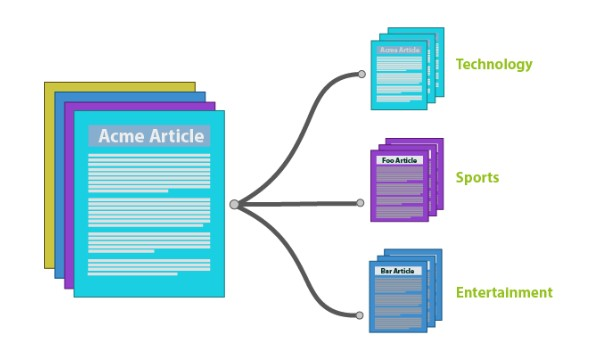
\includegraphics[scale=0.5]{figures/m1.jpg}
		\caption{Lusia-Klasifikasi teks}
		\label{contoh}
	\end{figure}
	
\item Klasifikasi Bunga tidak dapat penggunakan machine learning
	\par Klasifikasi bunga tidak dapat menggunakan machine learning karena memiliki masalah input yang serupa namun output yang berbeda atau 'noise'. Yang dimaksud dengan noise adalah contoh output yang direkam bukan seperti seharusnya. Misalnya saja kita secara implisit berasumsi bahwa contoh bunga kita telah diklasifikasikan dengan benar. Tetapi ini harus dilakukan dengan seseorang yang tepat, seperti seorang ahli botani. Seorang ahli botani ahli harus melihat contoh bunga dan berkata: " ini adalah setosa ... ini adalah virginica ", dan dengan demikian bertindak sebagai "guru" yang memungkinkan mesin untuk belajar. Tetapi bagaimana jika guru itu melakukan kesalahan? Selain itu, selalu ada peluang untuk memperkenalkan kesalahan saat merekam data. Noise juga ditemukan dalam pengukuran, yang selalu sedikit bermasalah karena alat dan sensor kami tidak sempurna dan hanya bekerja pada tingkat presisi tertentu.
	\begin{figure}[ht]
		\centering
		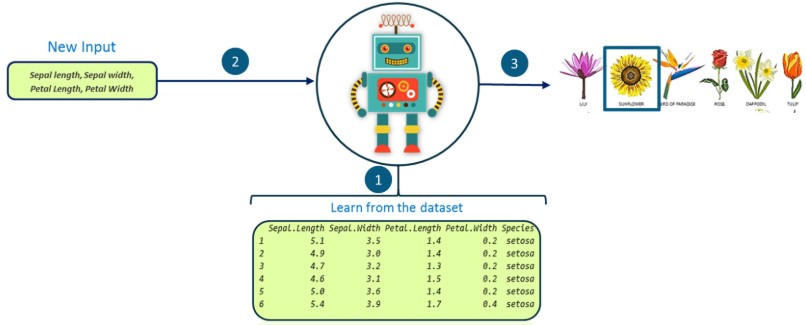
\includegraphics[scale=0.5]{figures/m2.jpg}
		\caption{Lusia-Klasifikasi bunga}
		\label{contoh}
	\end{figure}

\item Teknik pembelajaran mesin pada teks YouTube
	\par Dengan menggunakan kasus seperti rekomendasi video yang terdapat pada fiturnya, Machine Learning pada YouTube memperhatikan apa saja yang menarik perhatian para penggunanya. Ketika kita sedang menonton di YouTube, pada sebelah kanan terdapat 'Up Next' yang menampilkan beberapa video serupa yang sedang ditonton. Dan ketika mengklik salah satu video dari baris tersebut, maka YouTube akan mengingatnya dan menggunakan kata yang tertera sebagai referensi. 
	\begin{figure}[ht]
		\centering
		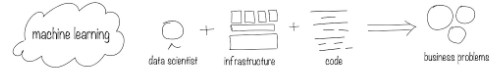
\includegraphics[scale=0.5]{figures/m3.jpg}
		\caption{Lusia-Teknik YouTube}
		\label{contoh}
	\end{figure}

\item Arti score
	\begin{itemize}
		\item Maksud arti score 44\% pada random forest adalah hasil akurasi.
		\item Maksud arti score 27\% pada decission tree adalah presentasi hasil dari perhitungan dataset.
		\item Maksud arti score 29\% dari SVM adalah hasil pendekatan neural network.
		\item Hasil tersebut didapat dari hasil valdasi silang untuk memastikan bahwa membagi  training test dengan cara yang berbeda. Sehingga didapat outputnya 44\% untuk hutan acak, 27\% untuk pohon keputusan, dan 29\% untuk SVM.
	\end{itemize}
	
\item Bag of word
	\par Bag-of-words adalah cara untuk merepresentasikan data teks saat memodelkan teks dengan algoritma pembelajaran mesin.
	\begin{figure}[ht]
		\centering
		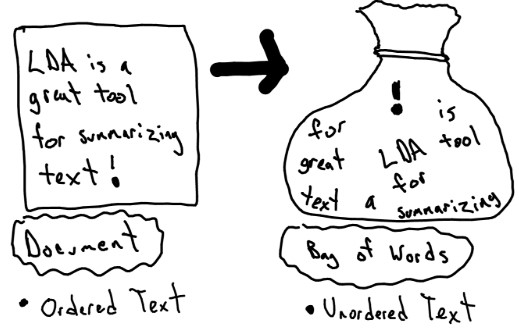
\includegraphics[scale=0.5]{figures/m5.jpg}
		\caption{Lusia-Bag of Word}
		\label{contoh}
	\end{figure}
	
\item TF-IDF
	\par TF-IDF merupakan istilah frekuensi - frekuensi dokumen terbalik, adalah ukuran penilaian yang banyak digunakan dalam pengambilan informasi (IR) atau peringkasan. TF-IDF dimaksudkan untuk mencerminkan seberapa relevan suatu istilah dalam dokumen yang diberikan. Intuisi di baliknya adalah bahwa jika sebuah kata muncul beberapa kali dalam sebuah dokumen, kita harus meningkatkan relevansinya karena itu harus lebih bermakna daripada kata-kata lain yang muncul lebih sedikit kali (TF). Pada saat yang sama, jika sebuah kata muncul berkali-kali dalam suatu dokumen tetapi juga di sepanjang banyak dokumen lain, mungkin itu karena kata ini hanya kata yang sering; bukan karena itu relevan atau bermakna (IDF).
	\begin{figure}[ht]
		\centering
		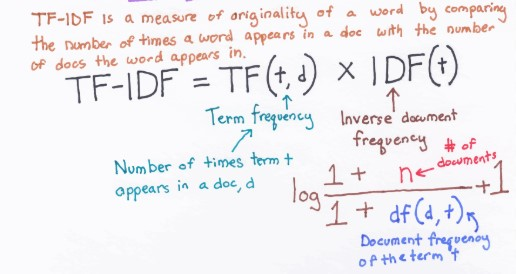
\includegraphics[scale=0.5]{figures/m6.jpg}
		\caption{Lusia-TF IDF}
		\label{contoh}
	\end{figure}
\end{enumerate}

\subsection{Praktek}